Any system can be regarded as some sort of "black box" or "machine" that turns a certain number of inputs into one or multiple output. Production systems do not escape that definition and can be viewed as a system transforming raw materials into final products. Actually, the inputs are more general and complex than just raw materials, for example, one can consider energy, workforce, decisions and many others as inputs of our system. As well, the outputs are generally not only a final product but also scraps or waste. Scrap corresponds to the portion of raw material that we loose with respect to the technology we utilize for transforming the raw materials into final products. Wastes, on the other hand, are immaterial. The figure (\ref{intro:production-system}) sums up what have been said.

\begin{figure}[h!]
    \centering
    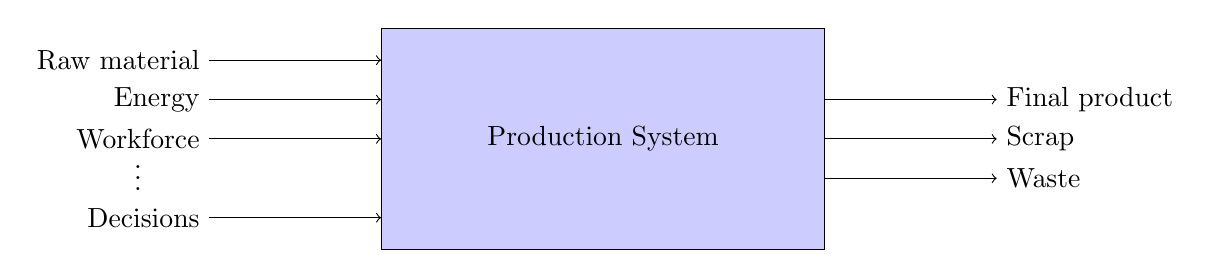
\begin{tikzpicture}
        % system
        \node[draw,fill=blue!20,minimum size=2em, minimum height=8em, minimum width=16em] at (0,0) (box) {Production System};

        % inputs
        \node at (-5, 1) (raw material) [left] {Raw material};
        \node at (-5, .5) (energy) [left] {Energy};
        \node at (-5, 0) (workforce) [left] {Workforce};
        \node at (-5, -1) (decisions) [left] {Decisions};

        % outputs
        \node at (5, .5) (final product) [right] {Final product};
        \node at (5, 0) (scrap) [right] {Scrap};
        \node at (5, -.5) (waste) [right] {Waste};

        % links
        \draw[->] (raw material) -- (raw material-|box.west);
        \draw[->] (energy) -- (energy-|box.west);
        \draw[->] (workforce) -- (workforce-|box.west);
        \draw[->] (decisions) -- (decisions-|box.west);
        \path (workforce) node (decisions) [below] {$\vdots$};

        \draw[<-] (final product) -- (final product-|box.east);
        \draw[<-] (scrap) -- (scrap-|box.east);
        \draw[<-] (waste) -- (waste-|box.east);
    \end{tikzpicture}
    \caption{\label{intro:production-system}General production system}
\end{figure}

The objective of this course is to analyse how we can make our production system more efficient with respect to some criteria (time, money, ...). Of course, our production depends on the methods and on the technolgies we use to manufacture our goods, but these are rather concerns for mechnanical engineers or more specific fields (chemistry, process engineering, ...). Actually, this course focuses on the only input we can, at our level, act uppon, which is : decisions.

To understand how decisions can improve (or worsen) our productivity, let's take a very simple example. Consider the following task : "Drilling four holes in a piece of wood". And let $X$ be the rate of production. Consider as well that the "drilling" operation needs some set-up time in order to prepare the right borer and to turn on the machine. Let's denote by $T_S$ this set-up time and by $T_H$ the operation time which is necessary to actually drill the wooden piece. There are plenty of ways to perform such task, one idea is to drill one hole at a time, stopping the machine after each drill. But this wouldn't be a very clever way since we would have to wait for the set-up time for each hole we want to make. Another idea is to perform a batch of holes in a row so that we only account for the set-up time once for all the batch. The two situations are presented in the GANT diagram in figure (\ref{intro:gant}).

\begin{figure}[h!]
    \centering
    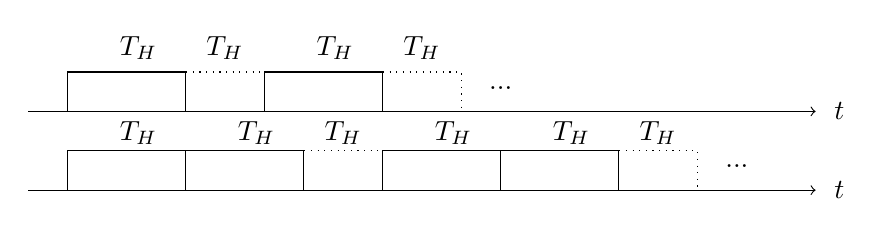
\begin{tikzpicture}
        % first gant
        \draw [->] (0,0) -- (10,0);
        \draw (10.3, 0) node {$t$};

        \draw (.5, 0) rectangle (2, .5);
        \draw (1.4, .8) node {$T_H$};

        \draw [dotted] (2, 0) rectangle (3, .5);
        \draw (2.5, .8) node {$T_H$};

        \draw (3, 0) rectangle (4.5, .5);
        \draw (3.9, .8) node {$T_H$};

        \draw [dotted] (4.5, 0) rectangle (5.5, .5);
        \draw (5, .8) node {$T_H$};

        \draw (6, .3) node {...};

        % second gant
        \draw [->] (0,-1) -- (10,-1);
        \draw (10.3, -1) node {$t$};

        \draw (.5, -1) rectangle (2, -.5);
        \draw (1.4, -.27) node {$T_H$};

        \draw (2, -1) rectangle (3.5, -.5);
        \draw (2.9, -.27) node {$T_H$};

        \draw [dotted] (3.5, -1) rectangle (4.5, -.5);
        \draw (4, -.27) node {$T_H$};

        \draw (4.5, -1) rectangle (6, -.5);
        \draw (5.4, -.27) node {$T_H$};

        \draw (6, -1) rectangle (7.5, -.5);
        \draw (6.9, -.27) node {$T_H$};

        \draw [dotted] (7.5, -1) rectangle (8.5, -.5);
        \draw (8, -.27) node {$T_H$};

        \draw (9, -.7) node {...};
        
    \end{tikzpicture}
    \caption{\label{intro:gant}Two GANT diagrams showing how decisions can influence productivity}
\end{figure}

In the first situation, the rate of production can be expressed as \[ X_1 = \frac{1}{T_H + T_S} \] meaning that we produce one item every $T_H+T_S$ unit of times. For the second situation however, the rate can be computed as \[ X_2 = \frac{2}{2T_H + T_S} = \frac{1}{T_H + \frac{T_S}{2}} \] which means that we produce one item every $T_H+\frac{T_S}{2}$ unit of time, which is smaller. In fact, as long as the batch size increases, the set-up time becomes less and less influent on the production rate since \[ X_k = \frac{k}{kT_H+T_S}\overset{k\rightarrow\infty}{\longrightarrow} \frac{1}{T_H} \] which clearly demonstrates that we can influence our production by making some decisions rather than others. 

The first part of this course will deal with the inventory management in which we'll try to answer to questions like "How and when should we order goods for our production system ?". In fact, we will deal with the different stakeholders to establish good strategies to make our orders. These stakeholders are represented in figure (\ref{intro:agents}). Firstly, the suppliers provides us with some raw materials which can then be stored in a warehouse. When needed, the production system will take some of these materials to transform them into final products. Once done, he will then leave them in another warehouse which will be used to fulfill the demand of such final goods. 

\begin{figure}[h!]
    \centering
    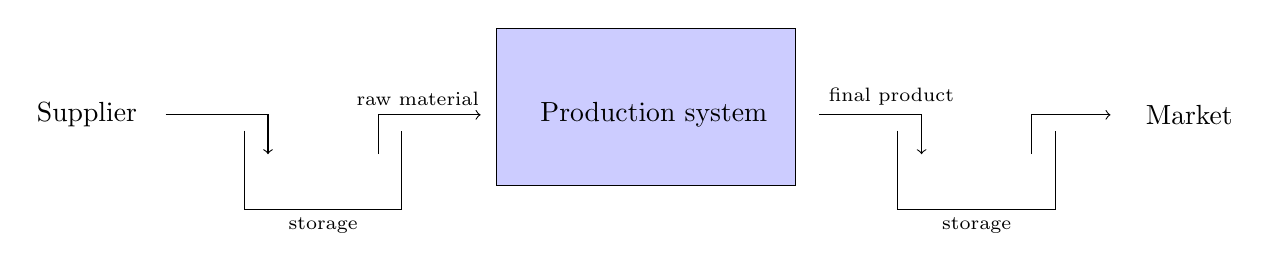
\begin{tikzpicture}
    % supplier -> storage
    \draw (0,0) -- (0,-1) -- (2, -1) -- (2, 0);
    \draw [->] (-1, .2) -| (.3, -.3);
    \draw (-2, .2) node {Supplier};
    \draw (1, -1.2) node {\scriptsize{storage}};

    % storage -> prod sys
    \draw [->] (1.7, -.3) |- (3, .2);
    \draw (1.3, .2) node [above right] {\scriptsize{raw material}};

    % prod sys
    \draw [fill=blue!20] (3.2, -.7) rectangle (7, 1.3);
    \draw (5.2, .2) node {Production system};

    % prod sys -> storage
    \draw [->] (7.3, .2) -| (8.6, -.3);
    \draw (7.3, .2) node [above right] {\scriptsize{final product}};
    
    
    % storage -> market
    \draw (8.3, 0) -- (8.3, -1) -- (10.3, -1) -- (10.3, 0);
    \draw [->] (10, -.3) |- (11, .2);
    \draw (12, .2) node {Market};
    \draw (9.3, -1.2) node {\scriptsize{storage}};

    \end{tikzpicture}
    \caption{\label{intro:agents}Production system agents}
\end{figure}

That being said, it is clear now that any production system aims to fulfill a certain demand taking into account the supply constraints it may encounter. This will be largely discussed futher on.

The figure (\ref{intro:system-types}) depicts the different production system types we can encounter :
\begin{itemize}
    \item Job shops : very specialized entities where, often, solely one product can be produced at the same time. Car repairers are a good example of such production systems. This kind of system is not easily formallized because they are too specific. We will not discuss them in this course. 
    \item Mass production : produces an average number of varieties of goods at average to high rate.
    \item Continuous flow process : produces continuously a given product at very high rate but with very small variety of products.
\end{itemize}

We will focus on both mass production and Continuous flow processes.

\begin{figure}[h!]
    \centering
    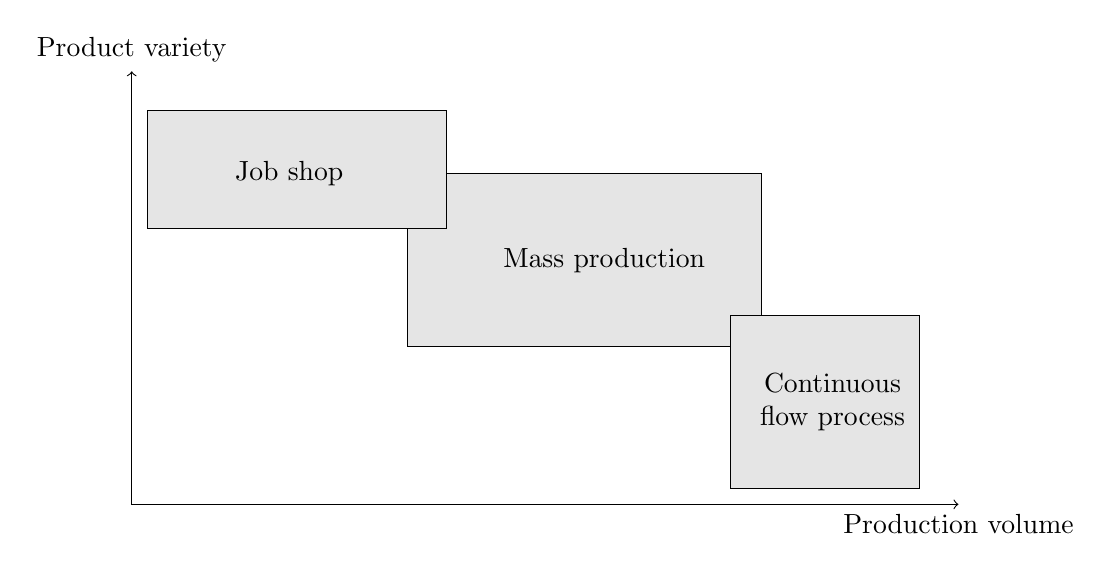
\begin{tikzpicture}
    % axis
    \draw [<->] (0,5.5) node (yaxis) [above] {Product variety} |- (10.5,0) node (xaxis) [below] {Production volume};

    \draw[fill=gray!20] (3.5, 2) rectangle (8, 4.2);
    \draw (6, 3.1) node {Mass production};

    \draw[fill=gray!20] (.2, 3.5) rectangle (4, 5);
    \draw (2, 4.2) node {Job shop};

    \draw[fill=gray!20] (7.6, 0.2) rectangle (10, 2.4);
    \draw [align=center] (8.9, 1.3) node {Continuous \\ flow process};

    \end{tikzpicture}
    \caption{\label{intro:system-types}Production system types}
\end{figure}

The second part of this course will take interest in the bill of materials (which will be further defined) in which we'll look at how to optimize production with respect to the production rate taking into account bottleneck machines in a production site. 